%amsart class
\documentclass[a4paper, 10pt, reqno]{amsart}

%Packages
\usepackage[utf8]{inputenc}
\usepackage[english]{babel}
\usepackage{graphics}
%\usepackage{graphicx}
\usepackage{subcaption}
\usepackage{physics}
\usepackage{listings}
\usepackage{hyperref}
\usepackage{blindtext}
\usepackage{xcolor}
\usepackage{pgf}
\usepackage{pgfplots}
\usepackage{placeins}
\usepackage{parskip}

\hypersetup{colorlinks=true, linkcolor=black, citecolor=black, urlcolor=blue}
%\hypersetup{hidelinks}

\pgfplotsset{compat=1.5}
\newlength\figureheight
\newlength\figurewidth
\setlength\figurewidth{0.98\textwidth}
\setlength\figureheight{0.75\figurewidth}

\usepackage{etoolbox}
\makeatletter
\patchcmd{\@maketitle}
  {\ifx\@empty\@dedicatory}
  {\ifx\@empty\@date \else {\vskip3ex \centering\footnotesize\@date\par\vskip1ex}\fi
   \ifx\@empty\@dedicatory}
  {}{}
\patchcmd{\@adminfootnotes}
  {\ifx\@empty\@date\else \@footnotetext{\@setdate}\fi}
  {}{}{}
\makeatother

%Custom colors
\definecolor{code}{rgb}{0.9, 0.17, 0.31}
\definecolor{coolgrey}{rgb}{0.55, 0.57, 0.67}
\definecolor{cyan(process)}{rgb}{0.0, 0.72, 0.92}
\definecolor{lightwhite}{rgb}{0.9647058823529412, 0.9647058823529412, 0.9647058823529412}
\definecolor{royalblue}{rgb}{0.25, 0.41, 0.88}
\definecolor{mediumseagreen}{rgb}{0.24, 0.7, 0.44}
%listing customization
\lstset{ %
  backgroundcolor=\color{lightwhite},
  basicstyle=\ttfamily\footnotesize,        % the size of the fonts that are used for the code
  breakatwhitespace=true,         % sets if automatic breaks should only happen at whitespace
  breaklines=true,                 % sets automatic line breaking
  captionpos=b,                    % sets the caption-position to bottom
  commentstyle=\color{mediumseagreen},    % comment style
  deletekeywords={...},            % if you want to delete keywords from the given language
  escapeinside={\%*}{*)},          % if you want to add LaTeX within your code
  extendedchars=true,              % lets you use non-ASCII characters; for 8-bits encodings only, does not work with UTF-8
  frame=single,	                   % adds a frame around the code
  keepspaces=true,                 % keeps spaces in text, useful for keeping indentation of code (possibly needs columns=flexible)
  keywordstyle=\color{code},       % keyword style
  language=C++,                 % the language of the code
  otherkeywords={...},           % if you want to add more keywords to the set
  emph={int,char,double,float,unsigned,void,bool,RNG_int,agents,pow,fabs,RNG_real,C,Trade,arma,sort,DumpToFile },
  emphstyle={\color{royalblue}},
  rulecolor=\color{white},         % if not set, the frame-color may be changed on line-breaks within not-black text (e.g. comments (green here))
  numbers=left,
  showspaces=false,                % show spaces everywhere adding particular underscores; it overrides 'showstringspaces'
  showstringspaces=false,          % underline spaces within strings only
  showtabs=false,                  % show tabs within strings adding particular underscores
  stepnumber=1,                    % the step between two line-numbers. If it's 1, each line will be numbered
  tabsize=3,	                   % sets default tabsize to 2 spaces
}

%Frontpage stuff
\title[Compulsory Assignment 1]{\Large{Compulsory Assignment 1}\\
\normalsize{STK4900 - Statistical methods and applications}}

\author[Metin San]{Metin San}
\date{\today}



%Begining document
\begin{document}

\maketitle

\section{Introduction}
This is the first of two compulsory assignment to be handed in in the course STK4900. It consists of two individual exercises. The first exercise considers an air pollution study made by the Norwegian Public Roads Administration, while the second exercise is a study of blood pressure in men. In the main part of the report, we will present and discuss the results of both studies in addition to looking at what the learning outcome of the studies are. The numerical code used to obtain the results and statistical quantities are attached in an appendix at the end of the report.


\section{Exercise 1: Air Pollution Study}
In this exercise we will look closer at a study made by the Norwegian Public Roads Administration. The study considers the air pollution at a measuring station at Alnabru in Oslo. The air pollution is measured by the NO$_2$ concentration. The data set consists of 500 observations of the following variables

\begin{itemize}
    \item Logarithm of NO$_2$ concentration
    \item Logarithm of number of cars per hour
    \item Temperature 2 meters about ground level [degrees C]
    \item Wind speed [meters/second]
    \item Hours of the day where the measurements were collected (1-24)
\end{itemize}

\subsection{a)}
We start by looking at the two variables log.no2 and log.cars. A summary from R yields the follow results seen in table \ref{tab: summary}. 

\begin{table}[h]
\caption{Main features of the variables log.no2 and log.cars as summarized by R through the summary command.}
\label{tab: summary}
\begin{tabular}{lllllll}
\hline\hline
Variable & Min.  & 1st Qu. & Median & Mean  & 3rd Qu. & Max.  \\ \hline
log.no2 & 1.224 & 3.214   & 3.848  & 3.698 & 4.217   & 6.395 \\
log.cars   & 4.127 & 6.176   & 7.425  & 6.973 & 7.793   & 8.349\\
\hline
\end{tabular}
\end{table}

These numerical values can also be shown through boxplots as seen in figure \ref{fig: boxplot}, which give a nice summary of the variables. The line that dives the boxes in two represents the median of the data. The 1st and 2nd quartiles are represented as the upper and lower ends of the boxes respectively.

\begin{figure}
    \centering
    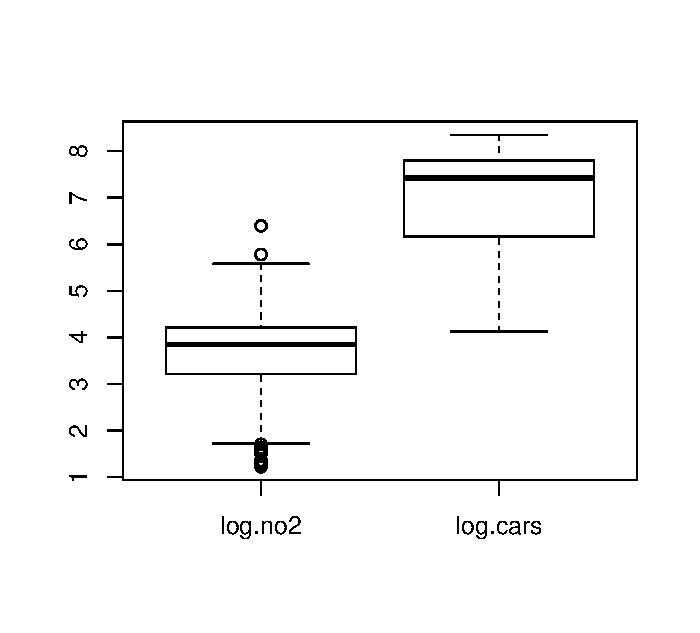
\includegraphics[width = 0.7\textwidth]{boxplot.pdf}
    \caption{Boxplot of the two variables log.no2 and log.cars.}
    \label{fig: boxplot}
\end{figure}

We proceed by plotting a scatterplot with log.cars as the x-axis and log.no2 as the y-axis. The results are seen in figure \ref{fig: log.no2log.cars}. We observe an increase in air pollution with increasing number of cars as expected. It should be noted that the values are logged, resulting in a less apparent visual increase. We also see that the scatterpoints are concentrated according to both variables median, as seen in table \ref{tab: summary}. The shape of the scatter distribution also suggests a correlation between the two variables.

\begin{figure}[h]
    \centering
    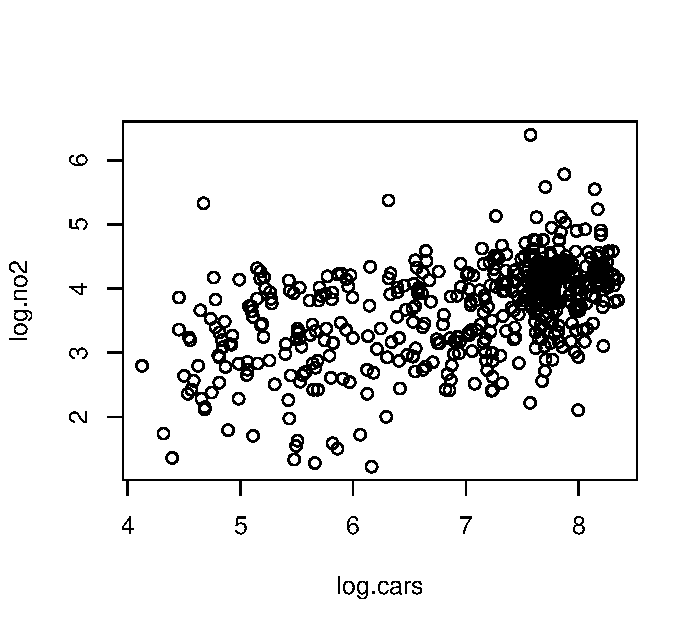
\includegraphics[width = 0.7\textwidth]{cor_log2nologcars.pdf}
    \caption{Scatterplot of log.no2 as a function of log.cars.}
    \label{fig: log.no2log.cars}
\end{figure}

\subsection{b)}
We will now fit a simple linear model where the concentration of NO$_2$ is explained by the traffic (cars per hour). The simplest linear regression is given by
\begin{equation}\label{eq: linreq}
    y_i = \beta_0 + \beta_1 x_i + \varepsilon_i,
\end{equation}
where $i = 1,...,n$ and $y_1,...,y_n$ are the response (outcomes), while $x_1,...,x_n$ are the predictors (variables). The coefficient $\beta_0$ represents the intersection, while $\beta_1$ determines the slope of the response. The $\varepsilon_i$ represent the random error (noise) in the model.

Numerically this is implemented through the lm.fit function in R. The coefficients of the linear fit along with a summary is given in table \ref{tab: linfit}.

\begin{table}[h]
\caption{Coefficients of the simple linear model used to fit the data in figure \ref{fig: log.no2log.cars}. The linear fit results in a $R^2$: 0.2622, and a adjusted $R^2$: 0.2607.}
\label{tab: linfit}
\begin{tabular}{lllllll}
\hline\hline
 & Esitmate Std.  & Error & t value & Pr$(>\abs{\mathrm{t}})$ & \\ \hline
(Intercept) & 1.23310 & 0.18755   & 6.575  & 1.23e-10 & ***\\
log.cars   & 0.35353 & 0.02657   & 13.303  & $<$ 2e-16 & ***\\
\hline
\end{tabular}
\end{table}

From table \ref{tab: linfit} we see that our model results in the following coefficients: $\beta_0 = 1.2331$ and $\beta_1 = 0.3536$, meaning that our linear regression model becomes
\begin{equation}
    \mathrm{log.no2} = 1.2331 + 0.3535\mathrm{log.cars} + \epsilon.
\end{equation}
We proceed by plotting the linear fit together with the scatterplot. The results of this can be seen in figure \ref{fig: linfit}.
\begin{figure}[h]
    \centering
    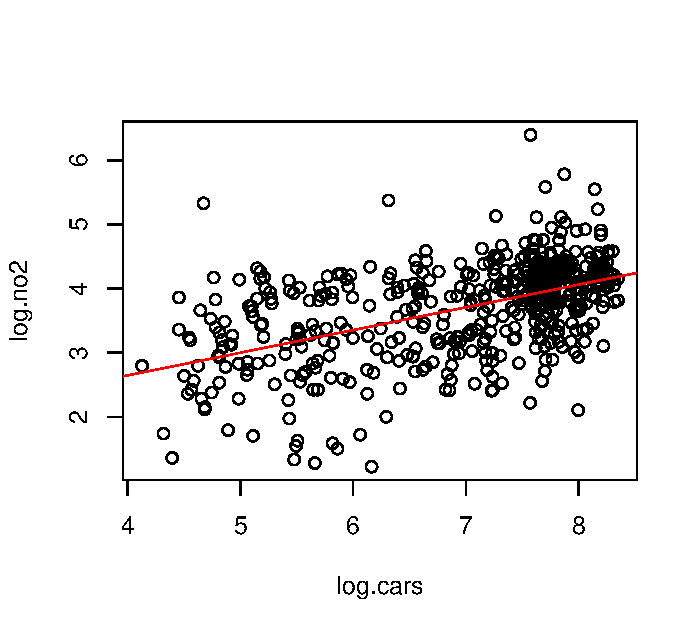
\includegraphics[width = 0.7\textwidth]{linfit.pdf}
    \caption{Scatterplot of log.no2 as a function of log.cars. The red line represents the simple linear fit seen in table \ref{tab: linfit}.}
    \label{fig: linfit}
\end{figure}
The coefficient of determination, also known as $R^2$ (mentioned in the caption of table \ref{tab: linfit}) provides a measure of how well the observed outcomes are replicated by our model. For a simple linear model such as the one we are considering, we have the relation
\begin{equation}
    R^2 = r^2,
\end{equation}
where $r^2$ is the square of the Pearson correlation coefficient which measures the linear correlation between two variables. From R, we find the Pearson correlation coefficient $r = 0.5121$ for the two variables log.no2 and log.cars. Squaring this gives us $r^2 = R^2 = 0.2622$, which is exactly equal to the $R^2$ found from the linear model. The value of $R^2$ tells us that there are indeed some correlation between these parameters, but the magnitude is not very convincing. This might be a result of us not considering other predictors which might be correlated.

\subsection{c)}
We will now look at the assumptions made for the linear regression model in 1b). For a general model given as
\begin{equation}
    y_i = \eta_i + \varepsilon_i,
\end{equation}
where $\eta_i$ represents the systematic part, and $\varepsilon_i$ the random (error). The 4 assumptions for linear regresion are then
\begin{enumerate}
    \item Linearity:
    \begin{equation}
        \eta_i = \beta_0 + \beta_1 x_{1i} + \beta_2 x_{2i} + ... + \beta_p x_{pi}.
    \end{equation}
    \item Constant variance (homoscedasticity):
    \begin{equation}
        \operatorname{Var}\left(\varepsilon_{i}\right)=\sigma_{\varepsilon}^{2} \qquad \forall \quad  i.
    \end{equation}
    \item Normally distributed errors:
    \begin{equation}
        \varepsilon_{i} \sim N\left(0, \sigma_{\varepsilon}^{2}\right).
    \end{equation}
    \item Uncorrelated errors:
    \begin{equation}
        \operatorname{Cov}\left(\varepsilon_{i}, \varepsilon_{j}\right)=0 \qquad \forall \quad  i \neq j.
    \end{equation}
\end{enumerate}
We will focus one the 3 first assumptions. We start by checking the linearity of our model. By using the "car" library in R, we can make a CPR (component-plus-residual) plot which is seen in figure \ref{fig: linearity}.
\begin{figure}
    \centering
    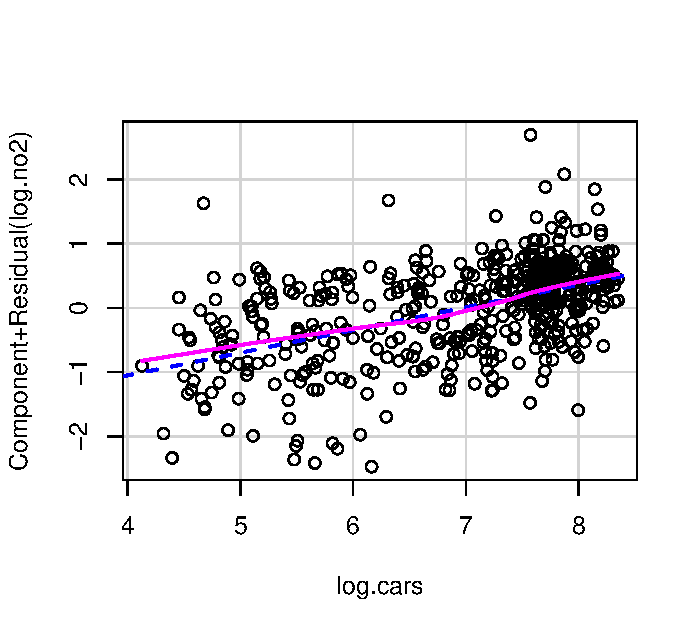
\includegraphics[width = 0.7\textwidth]{linearity.pdf}
    \caption{Component-plus-residual plot of the predictor log.cars.}
    \label{fig: linearity}
\end{figure}
The plot indicates that a linear function is the appropriate choice. 

We proceed by checking the homoscedasticity of the model. We find the following results by plotting the residuals and the square root of the standardized residuals as functions of the fitted values seen in figure \ref{fig: homo}. From the figure, we see that the variance is relatively constant with some deviation around the fitted value 3.5.

\begin{figure}
    \centering
    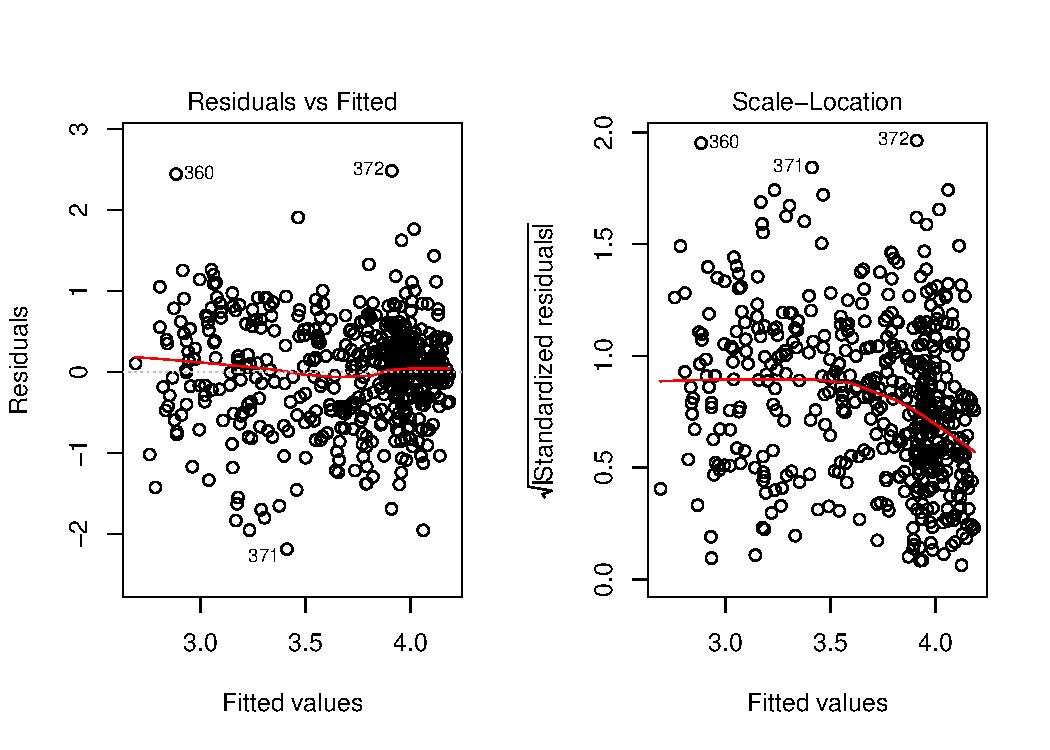
\includegraphics[width = 0.8\textwidth]{homo.pdf}
    \caption{Residual and the square root of the standardized residuals plotted as fucntions of the fitted values.}
    \label{fig: homo}
\end{figure}

Finally, we check the normality of the model. Using R, we make a histogram, a boxplot and a Q-Q plot of the fitted residuals. The results are seen in the figures \ref{fig: histbox} and \ref{fig: qq}. The histogram suggests that the distribution is relatively normal, and the shape is somewhat Gaussian. From the Q-Q plot we see that the sample quantiles mostly follow a straight line, meaning that they are mostly normal. They deviate from the straight line at the edges which is also seen in the box plot. To conclude, the assumptions made seem to coincide with the results, and the model could be described by a linear regression.

\begin{figure}
    \centering
    \begin{subfigure}{0.48\textwidth}
        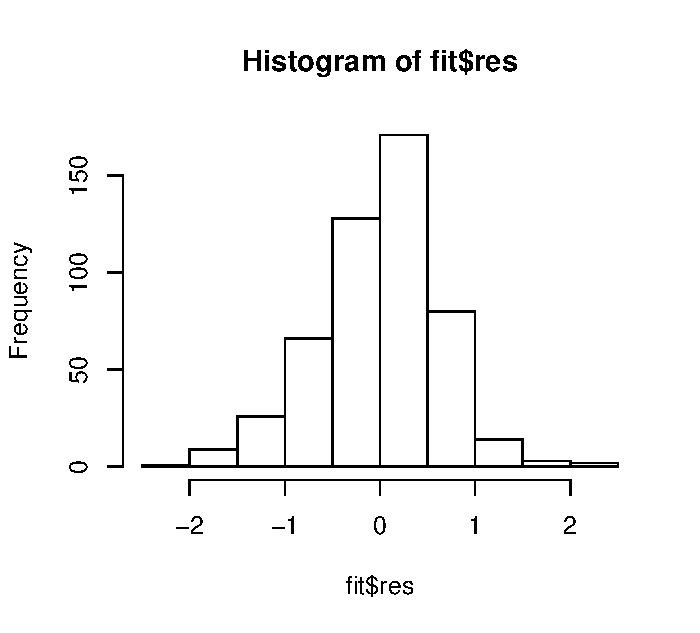
\includegraphics[width = \textwidth]{hist.pdf}
    \end{subfigure}
    ~
    \begin{subfigure}{0.48\textwidth}
        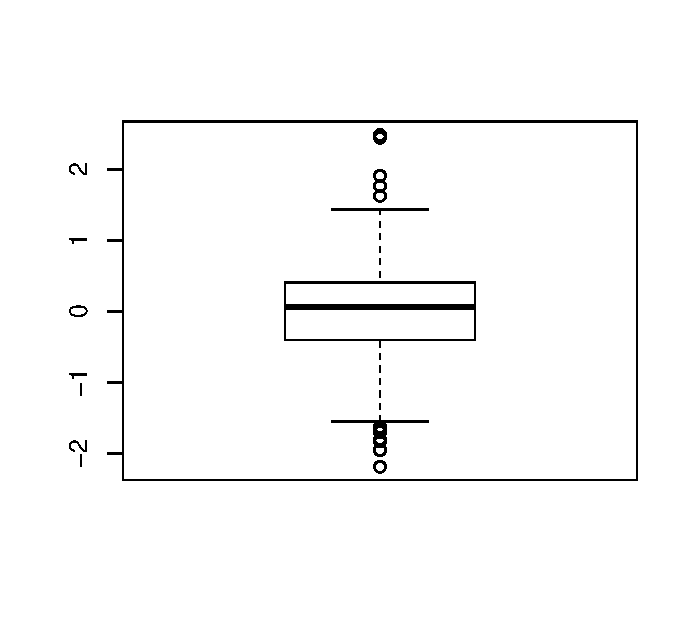
\includegraphics[width = \textwidth]{boxplotres.pdf}
    \end{subfigure}
    \caption{Histogram and boxplot demonstrating normality.}
    \label{fig: histbox}
\end{figure}

\begin{figure}
    \centering
    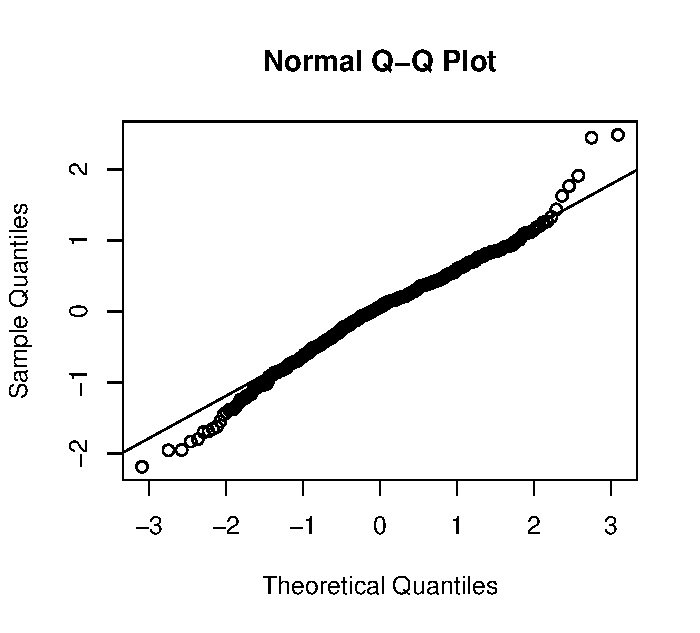
\includegraphics[width = 0.8\textwidth]{qqplot.pdf}
    \caption{QQ plot for the simple linear model demonstrating the linearity.}
    \label{fig: qq}
\end{figure}

\subsection{d)}
We proceed by using multiple regression to study the simultaneous effect of the various predictors. We start by checking the correlation between predictors. This is done in order to not include highly correlated predictors which would both increase the standard error of the correlated variables in addition to reducing the significance of one of them. By doing this we find that the covariates log.cars and log.hour.per.day are by far the highest correlated predictors with a correlation of 0.5769. A multilinear model including all predictors results in summary seen in table \ref{tab: multilin all}.


\begin{table}
\caption{Coefficients of the multi linear regression including all predictors. Multiple R-squared:  0.4807,	Adjusted R-squared:  0.4766 }
\label{tab: multilin all}
\begin{tabular}{lllllll}
\hline\hline
 & Esitmate  & Std. Error & t value & Pr$(>\abs{\mathrm{t}})$ & \\ \hline
(Intercept) & 1.111953 & 0.169410   & 6.564  & 1.33e-10 & ***\\
log.cars   & 0.461040 & 0.031041   & 14.852  & $<$ 2e-16 & ***\\
log(wind.speed) &  -0.415333 &  0.036410 & -11.407 & $<$ 2e-16 &***\\
log(hour.of.day) & -0.098007  & 0.041880 & -2.340 &  0.0197 &*\\
Temperature &            -0.026922  & 0.003853 & -6.988 &9.07e-12& ***\\
\hline
\end{tabular}
\end{table}

\begin{table}
\caption{Coefficients of the multi linear regression including not including the log(hour.per.day) predictor. Multiple R-squared:  0.475,	Adjusted R-squared:  0.4718  }
\label{tab: multilin}
\begin{tabular}{lllllll}
\hline\hline
 & Esitmate  & Std. Error & t value & Pr$(>\abs{\mathrm{t}})$ & \\ \hline
(Intercept)& 1.229009  & 0.162586  & 7.559 &1.98e-13 &***\\
log.cars   &0.411979&   0.022995  &17.916 & $<$ 2e-16& ***\\
log(wind.speed)& -0.414496  & 0.036572 &-11.334 & $<$ 2e-16 &***\\
Temperature &-0.026304  & 0.003861 & -6.813& 2.79e-11& ***\\
\hline
\end{tabular}
\end{table}

From the table (caption) we see that the $R^2$ has significantly increased. We can perform the same regression without the log(hour.per.day) variable. This gives us the results seen in table \ref{tab: multilin}. We see that the $R^2$ is slightly smaller for the model without the hour.of.day predictor. This is expected as more predictors will almost always result in a higher $R^2$. We also observe that the standard error of log.cars has gone down slightly. It should be noted that we have log transformed both hour.of.day and wind.speed to better match the other quantities. The temperature however contains negative values making a log transformation impossible.

The final model is the one without the predictor hour.of.day. A CPR plot of the model is seen in figure \ref{fig: multi cpr} where we observe a good linearity in all the covariates.

\begin{figure}[h]
    \centering
    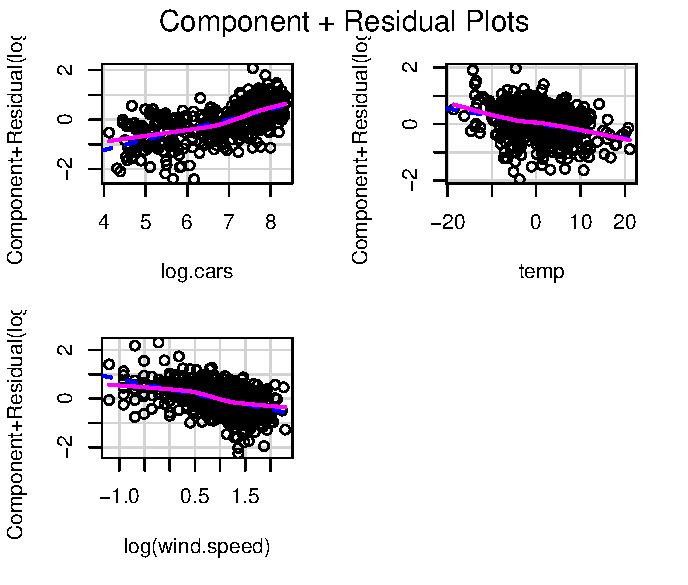
\includegraphics[width = 0.8\textwidth]{multicpr.pdf}
    \caption{CPR plot of the final multi linear model.}
    \label{fig: multi cpr}
\end{figure}

\subsection{e)}
The coefficients of the mulitlinear model represents the mean change in the response variable (air pollution) for one unit of change in the predictor variable while the other predictors are held constant. The coefficients can be thought of as the slope of the plot. Our model results in the coefficients seen in table \ref{tab: multilin}. We see that the coefficient for the predictor log.cars is 0.412. This means that for every unit increase in log.cars, we expect an increase in log.no2 by 0.412. The same interpretation is also valid for the other variables. We not that both log(wind.speed) and temperature has negative coefficients. This means that they help to lower the air pollution. We observe that the magnitude of the coefficients for log.cars and log(wind.speed) are very similar, meaning that they play an equally important role in observed air pollution. The effect of the coefficients can be seen in the CPR plot in figure \ref{fig: multi cpr}.

\section{Exercise 2: Blood Pressure}
In this exercise, we will look at a study considering the blood pressure of 36 random men. These men are divided into three age groups ranging from 30 to 75 years. The data can be seen in table \ref{tab: blood}.
\begin{table}[h]
    \caption{Measurements of blood pressure of random samples of 12 men in three different age groups.}
    \label{tab: blood}
    \begin{tabular}{|c|c|c|c|c|}
        \hline \hline 
        30-45 years  & 46-59 years & 60-75 years \\ 
        \hline 128, 104, 132, 112 & 120, 136, 174, 166 & 214, 146, 138, 148 \\ 
        \hline 136, 124, 112, 118 & 138, 124, 160, 157 & 156, 110, 188, 158 \\
        \hline 116, 108, 160, 116 & 108, 110, 154, 122 & 182, 148, 138, 136 \\ 
        \hline\hline 
    \end{tabular}
\end{table}
\subsection{a)}
We start by making a summary of the blood pressure of each age category. This is done in R, and the results are seen in table \ref{tab: bloodsum}. From the summary, we find that there appears to be a convincing correlation between age and blood pressure. All statistical quantities increase with age. We can also make a boxplot which describes the same numerical summaries. This can be seen in figure \ref{fig: bloodbox}. 

It is also interesting to note that group 1 have the most concentrated blood pressure out of all groups, suggesting that younger people have a relatively stable levels of blood pressure with the exception of the one person with 160 in blood pressure. Since the subjects are picked out at random, it is to be expected that there will be some outliers. We also observe that group 3 has the widest range of blood pressure.


\begin{table}
\caption{Numerical summary of the 3 different age groups.}
\label{tab: bloodsum}
\begin{tabular}{lllllll}
\hline\hline
Age group   & Min.  & 1st Qu. & Median & Mean  & 3rd Qu. & Max.  \\ \hline
30-45 years (1) & 104.0 & 112.0   & 117.0  & 122.2 & 129.0   & 160.0 \\
46-59 years (2)& 108.0 & 121.5   & 137.0  & 139.1 & 157.8   & 174.0 \\
60-75 years (3)& 110.0 & 138.0   & 148.0  & 155.2 & 164.0   & 214.0 \\ \hline
\end{tabular}
\end{table}

\begin{figure}
    \centering
    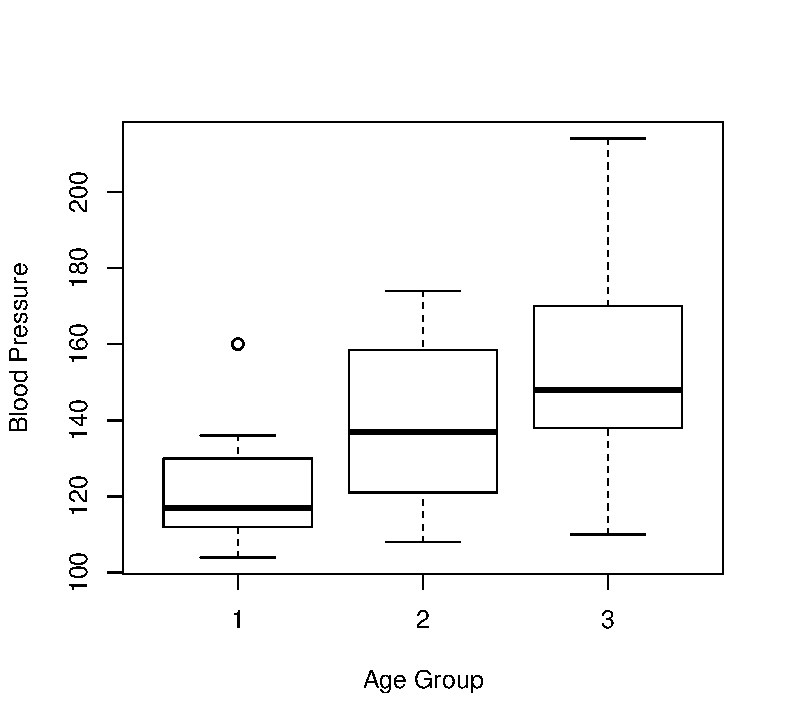
\includegraphics[width = 0.8\textwidth]{bloodbox.pdf}
    \caption{Boxplot showing the numerical statistical values of each age group.}
    \label{fig: bloodbox}
\end{figure}

\subsection{b)}
We will now use a one-way analysis of variance (ANOVA) to check if blood pressure varies across age. A one-way ANOVA is used to determine whether there are any statistically significant differences between a set of independent groups. In general, when performing a ANOVA, one needs to assume that all observations are independent. In addition, observations from a group $k$ needs to be random samples from a normal distribution $N(\mu_k,\sigma^2)$ with mean $\mu_k$ and variance $\sigma^2$. We assume that this is the case for our study as we have chosen samples randomly. 

We start with the null hypothesis
\begin{equation}
    H_0: \mu_1 = \mu_2 = \mu_3,
\end{equation}
where $\mu_k$ is the mean blood pressure of group $k$. We are interested in testing this null hypothesis to see if $\mu_1 \neq \mu_2 \neq \mu_3$, meaning that age does play a role in blood pressure. Performing the ANOVA in R results in the following summary seen in table \ref{tab: anova} where Df is degrees of freedom, Sum Sq the sum of squares, Mean Sq the mean sum of squares, F is the test statistic which can then be used to compute the P-value Pr$(>F)$.  

\begin{table}
\caption{ANOVA results of the blood pressure study.}
\label{tab: anova}
\begin{tabular}{llllll}
\hline\hline
          & Df & Sum Sq & Mean Sq & F value & Pr(\textgreater{}F) \\ \hline
Age group & 2  & 6535   & 3268    & 6.469   & 0.00426             \\
Residuals & 33 & 16670  & 505     &         &\\       
\hline
\end{tabular}
\end{table}


The ANOVA results in a F value of 6.469 is of significant magnitude, suggesting that there are indeed some correlation between age and blood pressure. This means that we can reject the null hypotheses $H_0$.

\subsection{c)}
We will now reformulate the above problem using a regression model with age group as the categorical predictor. We will use treatment-contrast meaning that we age group 1 as reference, and we think of aging as the treatment. By running a linear fit with age group as categorical predictor in R, we find the following results seen in table \ref{tab: catelin}

\begin{table}
\caption{Summary of the regression model with age group as categorical predictor. Multiple R-squared:  0.2816,	Adjusted R-squared:  0.2381 }
\label{tab: catelin}
\begin{tabular}{lllllll}
\hline\hline
 & Esitmate  & Std. Error & t value & Pr$(>\abs{\mathrm{t}})$ & \\ \hline
(Intercept) & 122.167    &  6.488  &18.829&  $<$ 2e-16& ***\\
agegroup2 &    16.917   &   9.176 &  1.844 & 0.07423 &.  \\
agegroup3   &  33.000   &   9.176  & 3.596&  0.00104 &** \\
\hline
\end{tabular}
\end{table}

From these results, we see that the P-value from age group 2 is not that significant, when compared to that of age group 3. This could suggest that blood pressure increasingly affected by age in a non linear way. These result do also show that age is indeed a relevant factor for the blood pressure of men.

\section{Appendix}
Here follows the code for exercise 1 and 2


\lstinputlisting[language=R, firstline=1, lastline=63, caption={} , label=lst: equilibrium]{Oblig1.R}

\lstinputlisting[language=R, firstline=1, lastline=31, caption={} , label=lst: equilibrium]{Oblig1_2.R}

\nocite{*}
\bibliography{references}{}
\bibliographystyle{plain}
\end{document}

